\documentclass[11pt,a4paper]{article}
\usepackage[margin={2.6cm,2.6cm}]{geometry}
\usepackage{lmodern}
\usepackage{microtype}
\usepackage{enumitem}
\usepackage{array}
\usepackage[spanish,es-tabla]{babel}
\usepackage[utf8]{inputenc}
\usepackage[T1]{fontenc}
\usepackage{amsmath, amsthm, amsfonts}
\usepackage{hyperref}
\usepackage{xcolor}
\usepackage{graphicx}
 \usepackage{float}
\usepackage{listings}
\usepackage{fontawesome5}
\usepackage{dirtree}

\spanishdecimal{.}
\definecolor{azuluc}{HTML}{1F4E79}
\definecolor{grisclaro}{HTML}{F4F6F8}
\definecolor{gris}{HTML}{586069}
\definecolor{verde}{HTML}{2E7D32}
\definecolor{rojo}{HTML}{A94442}
\definecolor{git}{HTML}{F1502F}
\definecolor{morado_ubuntu}{RGB}{48, 10, 36}       % Fondo morado oscuro de Ubuntu GNOME
\definecolor{verde_ubuntu}{RGB}{78, 154, 6}        % Verde para comentarios
\definecolor{cyan_ubuntu}{RGB}{52, 226, 226}       % Cian para comandos
\definecolor{amarillo_ubuntu}{RGB}{250, 240, 190}  % Amarillo para cadenas
\definecolor{rojo_ubuntu}{RGB}{220, 50, 47}        % Rojo para errores
\definecolor{verde_claro_ubuntu}{RGB}{138, 226, 52} % Verde claro para el prompt
\definecolor{azul_ubuntu}{RGB}{114, 159, 207}      % Azul para símbolos y rutas
\definecolor{gris_ubuntu}{RGB}{128, 128, 128}      % Gris para el borde del frame
\definecolor{fondo_mac}{RGB}{255, 255, 250}       % Fondo beige claro típico de macOS
\definecolor{negro}{RGB}{0, 0, 0}                 % Texto en negro
\definecolor{verde_mac}{RGB}{63, 127, 95}         % Verde para comentarios
\definecolor{azul_mac}{RGB}{0, 0, 255}            % Azul para comandos y prompt
\definecolor{rojo_mac}{RGB}{196, 26, 22}          % Rojo para errores y cadenas
\definecolor{morado_mac}{RGB}{147, 39, 143}       % Morado para emphasis (opcional)
\definecolor{gris_mac}{RGB}{200, 200, 200}        % Gris para el borde del frame
\definecolor{DarkGreen}{RGB}{0,102,0}
\definecolor{DarkYellow}{RGB}{243,220,12}

\lstdefinestyle{rstyle}{
  language=R,
  basicstyle=\ttfamily\small,
  keywordstyle=\color{azuluc}\bfseries,
  commentstyle=\color{gris},
  stringstyle=\color{verde!70!black},
  showstringspaces=false,
  frame=single,
  rulecolor=\color{gris!30},
  backgroundcolor=\color{grisclaro},
  breaklines=true,
  showspaces=false,
  tabsize=2,
    literate=
    {á}{{\'a}}1
    {é}{{\'e}}1
    {í}{{\'i}}1
    {ó}{{\'o}}1
    {ú}{{\'u}}1
    {Á}{{\'A}}1
    {É}{{\'E}}1
    {Í}{{\'I}}1
    {Ó}{{\'O}}1
    {Ú}{{\'U}}1
    {ñ}{{\~n}}1
    {Ñ}{{\~N}}1
    {ü}{{\"u}}1
    {Ü}{{\"U}}1
    {¡}{{\textexclamdown}}1
	{`}{\textasciigrave}1 
    {´}{\textquotesingle}1,
}

\lstdefinestyle{rconsole}{
  language=R,
  basicstyle=\color{rojo}\ttfamily\small,
  showstringspaces=false,
  frame=single,
  rulecolor=\color{gris!30},
  breaklines=true,
  tabsize=2,
  literate=
    {á}{{\'a}}1
    {é}{{\'e}}1
    {í}{{\'i}}1
    {ó}{{\'o}}1
    {ú}{{\'u}}1
    {Á}{{\'A}}1
    {É}{{\'E}}1
    {Í}{{\'I}}1
    {Ó}{{\'O}}1
    {Ú}{{\'U}}1
    {ñ}{{\~n}}1
    {Ñ}{{\~N}}1
    {ü}{{\"u}}1
    {Ü}{{\"U}}1
    {¡}{{\textexclamdown}}1
	{`}{\textasciigrave}1 
    {´}{\textquotesingle}1,
}

\lstdefinestyle{routput}{
  language=R,
  basicstyle=\color{azuluc}\ttfamily\small,
  showstringspaces=false,
  frame=single,
  rulecolor=\color{gris!30},
  breaklines=true,
  tabsize=2,
  literate=
    {á}{{\'a}}1
    {é}{{\'e}}1
    {í}{{\'i}}1
    {ó}{{\'o}}1
    {ú}{{\'u}}1
    {Á}{{\'A}}1
    {É}{{\'E}}1
    {Í}{{\'I}}1
    {Ó}{{\'O}}1
    {Ú}{{\'U}}1
    {ñ}{{\~n}}1
    {Ñ}{{\~N}}1
    {ü}{{\"u}}1
    {Ü}{{\"U}}1
    {¡}{{\textexclamdown}}1
	{`}{\textasciigrave}1 
    {´}{\textquotesingle}1,
}

\lstdefinestyle{mdstyle}{
  basicstyle=\ttfamily\footnotesize,
  keywordstyle=\color{azuluc}\bfseries,
  commentstyle=\color{gris},
  showstringspaces=false,
  showspaces=false,
  tabsize=2,
  frame=single,
  rulecolor=\color{gris!30},
  backgroundcolor=\color{grisclaro},
  breaklines=true,
  breakatwhitespace=false,
  % Títulos Markdown
  morecomment=[l][\color{azuluc}\bfseries]{\#},
  % Enlaces y referencias
  morecomment=[s][\color{verde}]{(}{)},
  % Lenguajes utilizados en bloques de código
  classoffset=1,
    keywordstyle=\color{morado}\bfseries,
    morekeywords={python,bash,R,latex,json,yaml},
  classoffset=0,
  % Protocolos y enlaces
  emph={http,https,ftp},
  escapeinside={-@}{@-},
  emphstyle=\color{azuluc}\underbar,   
   literate=
    {á}{{\'a}}1
    {é}{{\'e}}1
    {í}{{\'i}}1
    {ó}{{\'o}}1
    {ú}{{\'u}}1
    {Á}{{\'A}}1
    {É}{{\'E}}1
    {Í}{{\'I}}1
    {Ó}{{\'O}}1
    {Ú}{{\'U}}1
    {ñ}{{\~n}}1
    {Ñ}{{\~N}}1
    {ü}{{\"u}}1
    {Ü}{{\"U}}1
    {¡}{{\textexclamdown}}1
	{`}{\textasciigrave}1 
    {´}{\textquotesingle}1,
}

\lstdefinestyle{ubuntugnome}{
  basicstyle=\ttfamily\small\color{white},
  backgroundcolor=\color{morado_ubuntu},
  commentstyle=\color{verde_ubuntu},
  keywordstyle=\color{cyan_ubuntu},
  stringstyle=\color{amarillo_ubuntu},
  emphstyle=\color{rojo_ubuntu},
  showstringspaces=false,
  frame=single,
  rulecolor=\color{gris_ubuntu},
  breaklines=true,
  postbreak=\mbox{\textcolor{white}{$\hookrightarrow$}\space},
  % Configuración para simular el prompt de Ubuntu
  upquote=true,
  % Resaltar el prompt de usuario
  emph={user@ubuntu:~\$},
  emphstyle={\color{verde_claro_ubuntu}\bfseries},
  % Resaltar errores (ej: "command not found")
  classoffset=1,
  emph={command not found,No such file or directory,Permission denied},
  emphstyle={\color{rojo_ubuntu}},
  classoffset=0,
}

\lstdefinestyle{macterminal}{
  basicstyle=\ttfamily\small\color{negro},
  backgroundcolor=\color{fondo_mac},
  commentstyle=\color{verde_mac},
  keywordstyle=\color{azul_mac},
  stringstyle=\color{rojo_mac},
  emphstyle=\color{morado_mac},
  showstringspaces=false,
  frame=single,
  rulecolor=\color{gris_mac},
  breaklines=true,
  postbreak=\mbox{\textcolor{negro}{$\hookrightarrow$}\space},
  % Configuración para simular el prompt de macOS
  upquote=true,
  % Resaltar el prompt de usuario
  emphstyle={\color{azul_mac}\bfseries},
  % Resaltar errores (ej: "command not found")
  classoffset=1,
  emph={command not found,No such file or directory,Permission denied},
  emphstyle={\color{rojo_mac}},
  classoffset=0
}

\lstdefinestyle{windowscmd}{
  basicstyle=\ttfamily\small\color{white},
  backgroundcolor=\color{black},
  showstringspaces=false,
  frame=single,
  rulecolor=\color{gris_mac},
  breaklines=true,
  postbreak=\mbox{\textcolor{negro}{$\hookrightarrow$}\space},
  % Configuración para simular el prompt de macOS
  upquote=true,
  % Resaltar el prompt de usuario
  emphstyle={\color{azul_mac}\bfseries},
  % Resaltar errores (ej: "command not found")
  classoffset=1,
  emph={command not found,No such file or directory,Permission denied},
  emphstyle={\color{rojo_mac}},
  classoffset=0
}

\newcommand*{\vsp}{\texttt{\textvisiblespace}} % visible space
\newcommand*{\strC}{\begingroup
  \obeyspaces
  \begingroup\lccode`~=`\ %
  \lowercase{\endgroup\let~}\vsp
  \dostrC}
\newcommand{\dostrC}[1]{\textnormal{{\slshape\ttfamily#1}}\endgroup} % string constant
\newcommand{\R}{\textcolor{azuluc}{\faIcon{r-project}}}
\newcommand{\Git}{\textcolor{git}{\faIcon{git-alt}}~\!Git}
\newcommand{\GitHub}{\faIcon{github}~\!GitHub}
\newcommand{\Markdown}{Markdown~\faIcon{markdown}}
\newcommand{\checkicon}{\textcolor{verde}{\faIcon{check}}}
\newcommand{\crossicon}{\textcolor{rojo}{\faIcon{times}}}
\newtheoremstyle{exercise}
  {0.8em}{0.8em}{\normalfont}{}{\bfseries\color{azuluc}}{.}{0.5em}{}
\theoremstyle{exercise}
\newtheorem{exercise}{Ejercicio}




\title{\LARGE\textbf{Práctica 8: Introducción al análisis estadístico con \R}\\[0.5em]
\Large Laboratorio de Matemáticas\\
\small\ \\
\Large Grado en Ingeniería Matemática - Doble Grado en Física e Ingeniería Matemática}
\author{Miguel Beltra Vidal}
\date{Curso 2026/27}
\begin{document}

\maketitle






\section{Objetivos}

El objetivo de esta práctica es aprender a importar, explorar, resumir y representar conjuntos de datos con \R. Se trabajará con variables cualitativas y cuantitativas, tanto por separado como conjuntamente. Al finalizar, el estudiante deberá ser capaz de construir tablas de frecuencias, calcular medidas descriptivas, elegir gráficos adecuados e interpretar relaciones entre variables. También aprenderá a documentar un análisis para que pueda reproducirse.


\section{Cargar datos en \R\ a partir de un fichero CSV}

Los archivos CSV (\emph{comma-separated values}) son un tipo de documento en formato abierto sencillo para representar datos en forma de tabla, en las que las columnas se separan por comas

\medskip

\begin{lstlisting}[style=mdstyle]
Año,Marca,Modelo,Descripción,Precio
1997,Ford,E350,"ac, ABS, moon",3000.00
1999,Chevy,Venture,Extended Edition,4900.00
1999,Chevy,Venture,"Extended Edition, Very Large",5000.00
1996,Jeep,Grand Cherokee,"MUST SELL! air, moon roof, loaded",4799.00
\end{lstlisting}

\medskip

\noindent Para importar un archivo CSV se puede usar \texttt{read.csv()}. 

\medskip

\begin{lstlisting}[style=rstyle]
datos <- read.csv("ruta/al/archivo.csv", fileEncoding = "UTF-8-BOM")
\end{lstlisting}

\medskip

El archivo cargado será un \texttt{data.frame}. Podemos utilizar las siguientes funciones para comprobar que los datos se han cargado correctamente: \texttt{names()} muestra los nombres de las columnas, \texttt{head()} las primeras filas, \texttt{str()} la estructura y los tipos de variables, y \texttt{summary()} un resumen inicial.

\medskip

\R\ también incluye algunos conjuntos de datos en la libreria \texttt{datasets}, incluida al instalar \R. A lo largo de toda la práctica utilizaremos el conjunto de datos \texttt{penguins} de \texttt{datasets}. Para cargarlos, utilizaremos la función \texttt{data()}.

\medskip

\begin{lstlisting}[style=rstyle]
data("penguins")
names(penguins)
head(penguins)
str(penguins)
summary(penguins)
\end{lstlisting}



\section{Librerías en \R}

\R\ incluye funciones básicas, pero muchas herramientas adicionales se distribuyen en paquetes. Para instalar un paquete se utiliza \texttt{install.packages()}, normalmente una sola vez en cada instalación de \R. Para utilizarlo en una sesión se carga con \texttt{library()}.

\medskip

\begin{lstlisting}[style=rstyle]
install.packages("faraway")  # solo la primera vez
library(faraway)             # cargar el paquete en la sesión
\end{lstlisting}

\medskip

\noindent Si el paquete ya está instalado, no es necesario volver a instalarlo. En cambio, hay que ejecutar \texttt{library(faraway)} cada vez que se inicia una nueva sesión en la que se quiera utilizar. Si queremos utilizar un conjunto de datos de una librería, lo podemos cargar también con \texttt{data()}. Por ejemplo, podemos cargar el conjunto de datos \texttt{Salaries} del paquete \texttt{faraway}.
\begin{lstlisting}[style=rstyle]
data(Salaries, package = "faraway")
\end{lstlisting}





\section{Variables cualitativas}

Las variables cualitativas (también llamadas categóricas) describen grupos o categorías. Una variable nominal no tiene un orden natural (por ejemplo, medio de transporte); una variable ordinal sí tiene un orden (por ejemplo, nivel de satisfacción bajo, medio o alto). Aunque una categoría se codifique con números, esos números no necesariamente representan cantidades medibles.

\subsection{Análisis numérico de variables cualitativas}

La función \texttt{table()} calcula las frecuencias absolutas de cada categoría. Con \texttt{prop.table()} se obtienen las frecuencias relativas, que pueden multiplicarse por 100 para expresarlas en porcentajes.
\begin{lstlisting}[style=rstyle]
table(penguins$species)
frecuencias <- table(penguins$species)
prop.table(frecuencias)
100 * prop.table(frecuencias)
\end{lstlisting}

En el ejemplo, sustituye \texttt{sex} por el nombre de la variable cualitativa que quieras estudiar. Si una variable cuantitativa tiene muchos valores diferentes, una tabla simple puede ser poco útil; en ese caso, agrupa los valores en intervalos.

\subsection{Representación gráfica de variables cualitativas}

\subsubsection{Gráficos de barras}

La función \texttt{barplot()} permite representar frecuencias o proporciones de diferentes categorías mediante un gráfico de barras. Primero se deberá calcular una tabla de frecuencias, que será la que reciba \texttt{barplot()} como argumento. Las barras aparecerán separadas al tratarse de categorías distintas. También se pueden utilizar algunos argumentos como los que estudiamos en la práctica de gráficos:

\begin{lstlisting}[style=rstyle]
barplot(frecuencias, 
        main = "Gráfico de barras: cantidad de pingüinos por especie",
        xlab = "Especie",
        ylab = "Cantidad",
        col = c("cyan","blue","darkblue"))
\end{lstlisting}

\begin{center}
	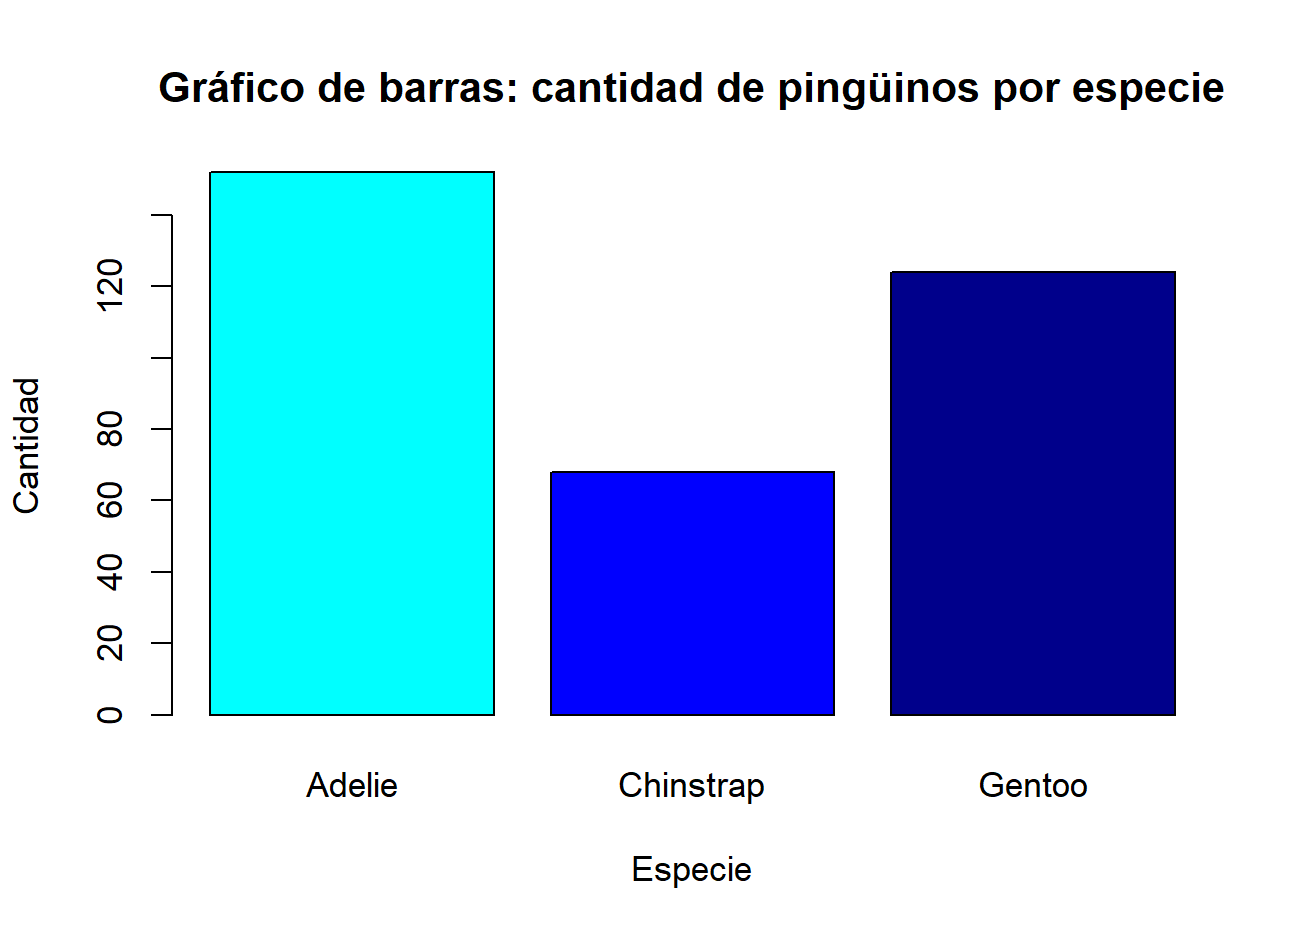
\includegraphics[width=0.5\linewidth]{images/barplot}
\end{center}

Puedes ver más detalles acerca de la función \texttt{barplot()} en el manual, ejecutando la siguiente instrucción en la consola de \R.

\begin{lstlisting}[style=rstyle]
> help(barplot)
\end{lstlisting}



\subsubsection{Gráficos de sectores}


La función \texttt{pie()} representa las proporciones de las categorías como sectores de un círculo. El tamaño de cada sector es proporcional a su frecuencia o porcentaje. Es más fácil de interpretar cuando hay pocas categorías; si hay muchas, suele ser preferible un gráfico de barras.

\begin{lstlisting}[style=rstyle]
pie(frecuencias,
    main = "Diagrama de sectores: cantidad de pingüinos por especie",
    col = c("cyan","blue","darkblue"))
\end{lstlisting}

\begin{center}
	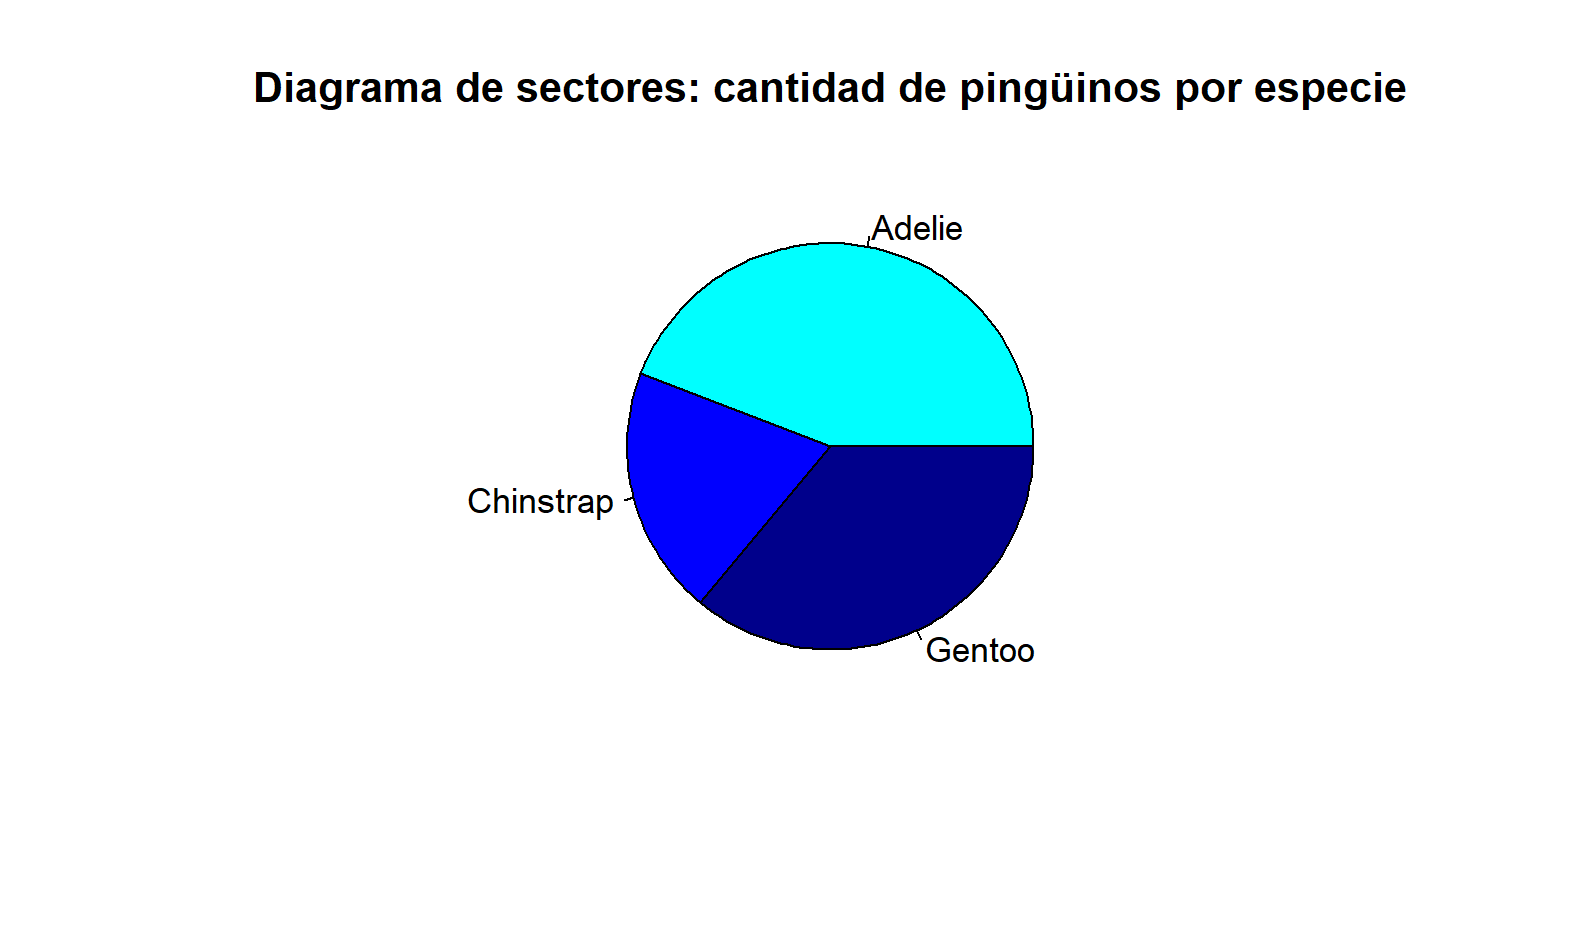
\includegraphics[width=0.75\linewidth]{images/pie}
\end{center}

Puedes ver más detalles acerca de la función \texttt{pie()} en el manual, ejecutando la siguiente instrucción en la consola de \R.

\begin{lstlisting}[style=rstyle]
> help(pie)
\end{lstlisting}



\section{Variables cuantitativas}

\subsection{Análisis numérico de variables cuantitativas}

Las funciones de la siguiente tabla nos permitirán realizar algunos de los cálculos más habituales de estadística descriptiva. El argumento \texttt{na.rm = TRUE} indica que los valores no asignados \texttt{NA} se deben remover a la hora de hacer el cálculo.

\begin{center}
	\begin{tabular}{|l|l|} \hline
		\textbf{Función} & \textbf{Descripción} \\ \hline	
		\texttt{mean(x, na.rm = TRUE)}     & media \\
		\texttt{median(x, na.rm = TRUE)}   & mediana \\
		\texttt{quantile(x, na.rm = TRUE)} & cuartiles y extremos \\
		\texttt{range(x, na.rm = TRUE)}    & mínimo y máximo \\
		\texttt{IQR(x, na.rm = TRUE)}      & rango intercuartílico \\
		\texttt{var(x, na.rm = TRUE)}      & varianza muestral (divisor $n-1$) \\
		\texttt{sd(x, na.rm = TRUE)}       & desviación típica muestral \\ \hline
	\end{tabular}
\end{center}

Las siguientes instrucciones:
\begin{lstlisting}[style=rconsole]
> mean(penguins$body_mass, na.rm=TRUE)
> median(penguins$body_mass, na.rm=TRUE)
> quantile(penguins$body_mass, na.rm=TRUE)
> range(penguins$body_mass, na.rm=TRUE)
> IQR(penguins$body_mass, na.rm=TRUE)
> var(penguins$body_mass, na.rm=TRUE)
> sd(penguins$body_mass, na.rm=TRUE)
\end{lstlisting}
tienen como salida los siguientes valores:
\begin{lstlisting}[style=routput]
[1] 4201.754
[1] 4050
  0%  25%  50%  75% 100% 
2700 3550 4050 4750 6300 
[1] 2700 6300
[1] 1200
[1] 643131.1
[1] 801.9545
\end{lstlisting}


\R\ también tiene algunas funciones de resumen que calculan muchos de los valores que hemos mencionado.

\begin{center}
	\begin{tabular}{|l|l|} \hline
		\textbf{Función} & \textbf{Descripción} \\ \hline	
		\texttt{summary(x)}                & mínimo, cuartiles, mediana y media \\
		\texttt{fivenum(x, na.rm = TRUE)}  & resumen de cinco números \\ \hline
	\end{tabular}
\end{center}


Por ejemplo, \texttt{summary()} tiene la siguiente salida:
\begin{lstlisting}[style=rconsole]
> summary(penguins$body_mass)
\end{lstlisting}
\begin{lstlisting}[style=routput]
   Min. 1st Qu.  Median    Mean 3rd Qu.    Max.     NAs 
   2700    3550    4050    4202    4750    6300       2 
\end{lstlisting}
mientras que \texttt{fivenum()} tiene la siguiente salida:
\begin{lstlisting}[style=rconsole]
> fivenum(penguins$body_mass, na.rm=TRUE)
\end{lstlisting}
\begin{lstlisting}[style=routput]
[1] 2700 3550 4050 4750 6300
\end{lstlisting}




La varianza que calcula \R\ es la muestral, que utiliza el divisor \(n-1\). Si se necesita la varianza de la población, esto es, con divisor \(n\), puede calcularse a partir de la anterior:
\begin{lstlisting}[style=rconsole]
> n <- sum(!is.na(penguins$body_mass))
> varianza_poblacional <- var(penguins$body_mass, na.rm=TRUE)*(n-1)/n
> desviacion_poblacional <- sqrt(varianza_poblacional)
> desviacion_poblacional
\end{lstlisting}
\begin{lstlisting}[style=routput]
[1] 800.7812
\end{lstlisting}

El coeficiente de variación mide la desviación típica en relación con el valor absoluto de la media; suele expresarse en porcentaje. No es adecuado si la media es cero o muy próxima a cero. \R\ no tiene una función específica para calcular este valor, pero es fácil calcularlo a partir de las funciones mencionadas anteriormente.
\begin{lstlisting}[style=rconsole]
> peso <- penguins$body_mass
> CV <- 100 * sd(peso, na.rm=TRUE)/abs(mean(peso, na.rm=TRUE))
> CV
\end{lstlisting}
\begin{lstlisting}[style=routput]
[1] 19.08618
\end{lstlisting}

La asimetría describe la falta de simetría de una distribución y la curtosis resume el peso relativo de sus colas. \R\ no tiene implementaciones de estas funciones. Para calcularlas se puede usar el paquete \texttt{moments}. Deberemos instalarlo (si no lo tenemos instalado) y cargarlo:
\begin{lstlisting}[style=rstyle]
install.packages("moments") # solo la primera vez
library(moments)
\end{lstlisting}
Una vez cargado el paquete, podemos utilizarlo:
\begin{lstlisting}[style=rconsole]
> skewness(penguins$body_mass, na.rm = TRUE)
\end{lstlisting}
\begin{lstlisting}[style=routput]
[1] 0.468264
\end{lstlisting}
\begin{lstlisting}[style=rconsole]
> kurtosis(penguins$body_mass, na.rm = TRUE)
\end{lstlisting}
\begin{lstlisting}[style=routput]
[1] 2.273757
\end{lstlisting}



La función \texttt{kurtosis()} de \texttt{moments} devuelve la curtosis de Pearson, cuyo valor de referencia para una distribución normal es 3. Los resultados de las distintas definiciones de asimetría y curtosis pueden variar ligeramente entre paquetes.


\subsection{Representación gráfica de variables cuantitativas}

Las medidas numéricas deben complementarse con gráficos, porque estos permiten detectar asimetrías, concentraciones, valores atípicos y posibles errores. El histograma muestra la distribución; el diagrama de caja resume mediana, cuartiles y posibles valores atípicos. Un diagrama de dispersión se utiliza cuando se estudian dos variables cuantitativas.


\subsubsection{Histogramas}

Los histogramas permiten estudiar cómo se distribuyen los valores de una variable numérica.

\begin{lstlisting}[style=rstyle]
hist(penguins$body_mass,
     main = "Histograma: peso de los pingüinos",
     xlab = "Peso",
     ylab = "Frecuencia",
     col = "gray")
\end{lstlisting}

\begin{center}
	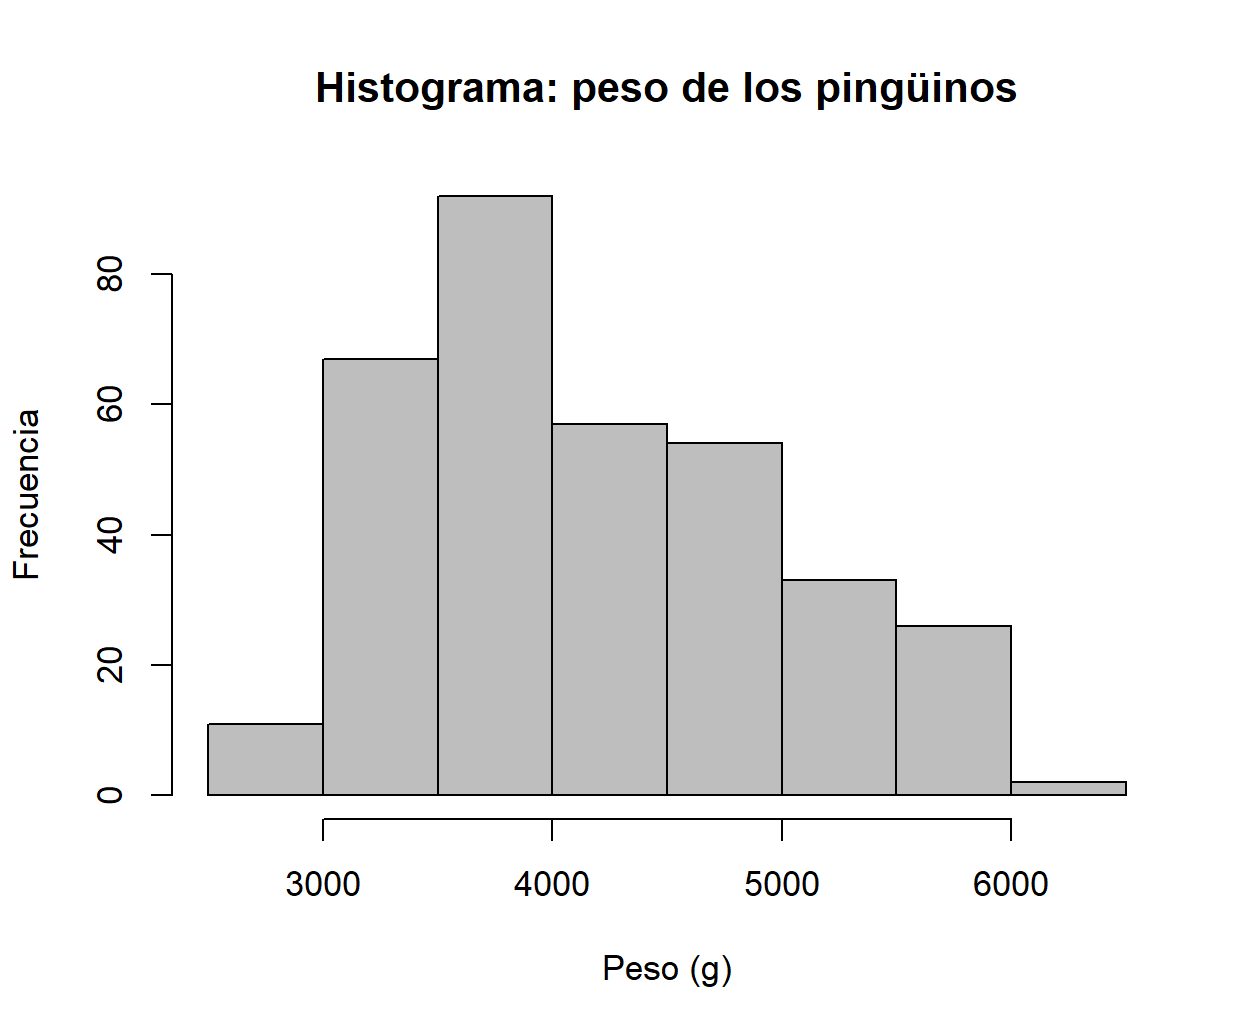
\includegraphics[width=0.6\linewidth]{images/hist}
\end{center}

Puedes ver más detalles acerca de la función \texttt{hist()} en el manual, ejecutando la siguiente instrucción en la consola de \R.

\begin{lstlisting}[style=rstyle]
> help(hist)
\end{lstlisting}


\subsubsection{Diagramas de caja}

El diagrama de caja (o gráfico de cajas y bigotes) resume una variable cuantitativa mediante sus cuartiles y su mediana. La caja abarca el primer y el tercer cuartil; la línea interior señala la mediana. Los bigotes suelen extenderse hasta los valores más extremos que no se consideran atípicos, y los puntos que quedan fuera se muestran como posibles valores atípicos. Este gráfico permite comparar la dispersión, la posición central y la presencia de valores extremos.

\begin{lstlisting}[style=rstyle]
boxplot(penguins$body_mass,
     main = "Diagrama de caja: peso de los pingüinos",
     ylab = "Peso (g)",
     col = "orange")
\end{lstlisting}

\begin{center}
	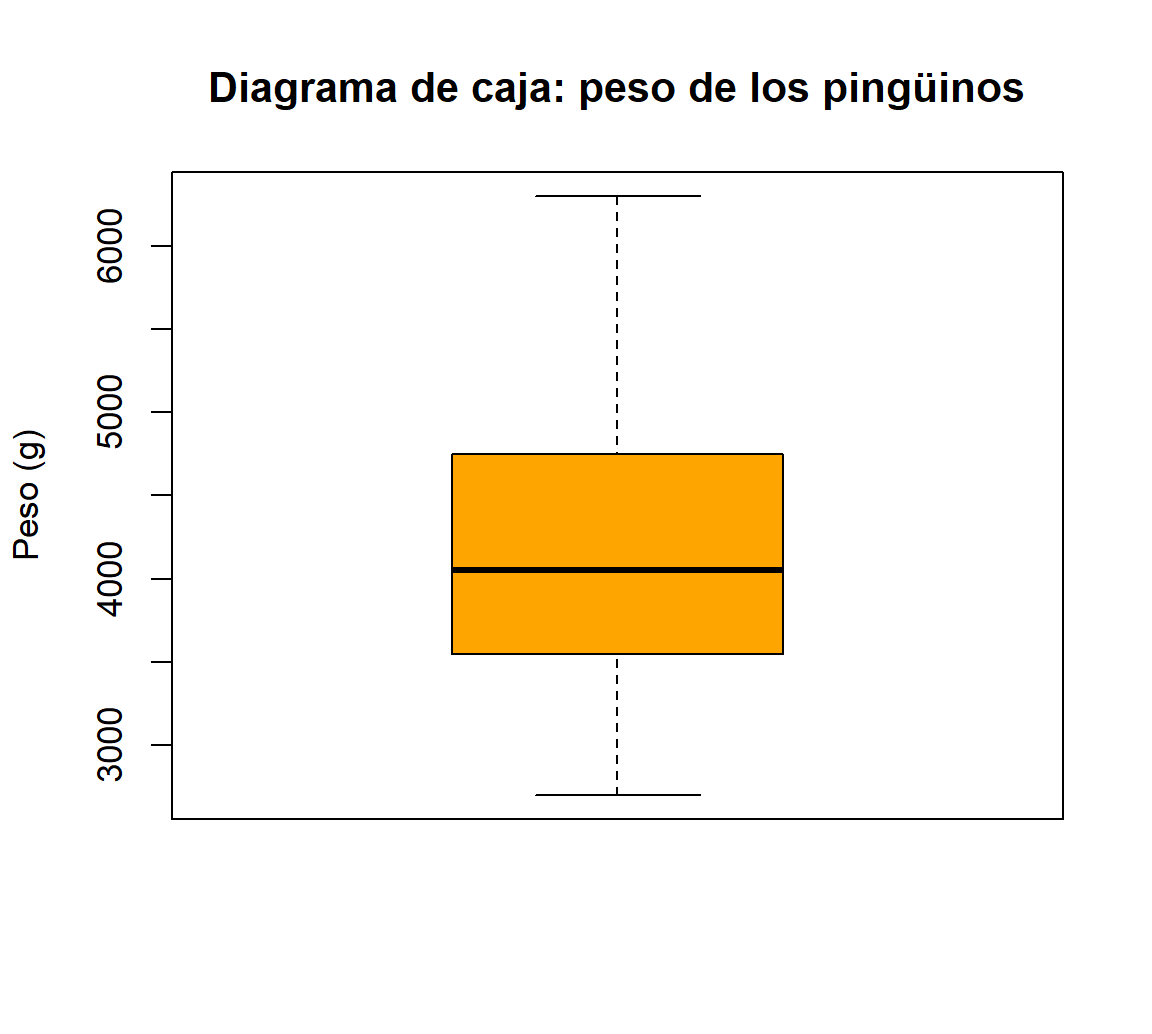
\includegraphics[width=0.45\linewidth]{images/boxplot}
\end{center}

Puedes ver más detalles acerca de \texttt{boxplot()} en el manual, con la siguiente instrucción:
\begin{lstlisting}[style=rstyle]
> help(boxplot)
\end{lstlisting}



\section{Análisis bivariante}

\subsection{Dos variables cualitativas}

Para estudiar dos variables cualitativas se construye una tabla de contingencia. Las filas representan las categorías de una variable y las columnas las de la otra.
\begin{lstlisting}[style=rstyle]
> tabla <- table(penguins$species, penguins$island)
> tabla
\end{lstlisting}

\begin{lstlisting}[style=routput]
            Biscoe Dream Torgersen
  Adelie        44    56        52
  Chinstrap      0    68         0
  Gentoo       124     0         0
\end{lstlisting}

\noindent Las frecuencias conjuntas pueden compararse con porcentajes por fila o por columna.

\begin{lstlisting}[style=rconsole]
> prop.table(tabla)
\end{lstlisting}

\begin{lstlisting}[style=routput]           
               Biscoe     Dream Torgersen
  Adelie    0.1279070 0.1627907 0.1511628
  Chinstrap 0.0000000 0.1976744 0.0000000
  Gentoo    0.3604651 0.0000000 0.0000000
\end{lstlisting}
  
  
\begin{lstlisting}[style=rconsole]
> 100*prop.table(tabla)
\end{lstlisting}
           
\begin{lstlisting}[style=routput]
              Biscoe    Dream Torgersen
  Adelie    12.79070 16.27907  15.11628
  Chinstrap  0.00000 19.76744   0.00000
  Gentoo    36.04651  0.00000   0.00000
\end{lstlisting}


\noindent Un gráfico de barras agrupadas o apiladas ayuda a visualizar las diferencias.

\begin{lstlisting}[style=rstyle]
barplot(tabla, 
        col = c("red","orange","brown"),
        beside = TRUE, 
        legend = TRUE)
\end{lstlisting}

\begin{center}
	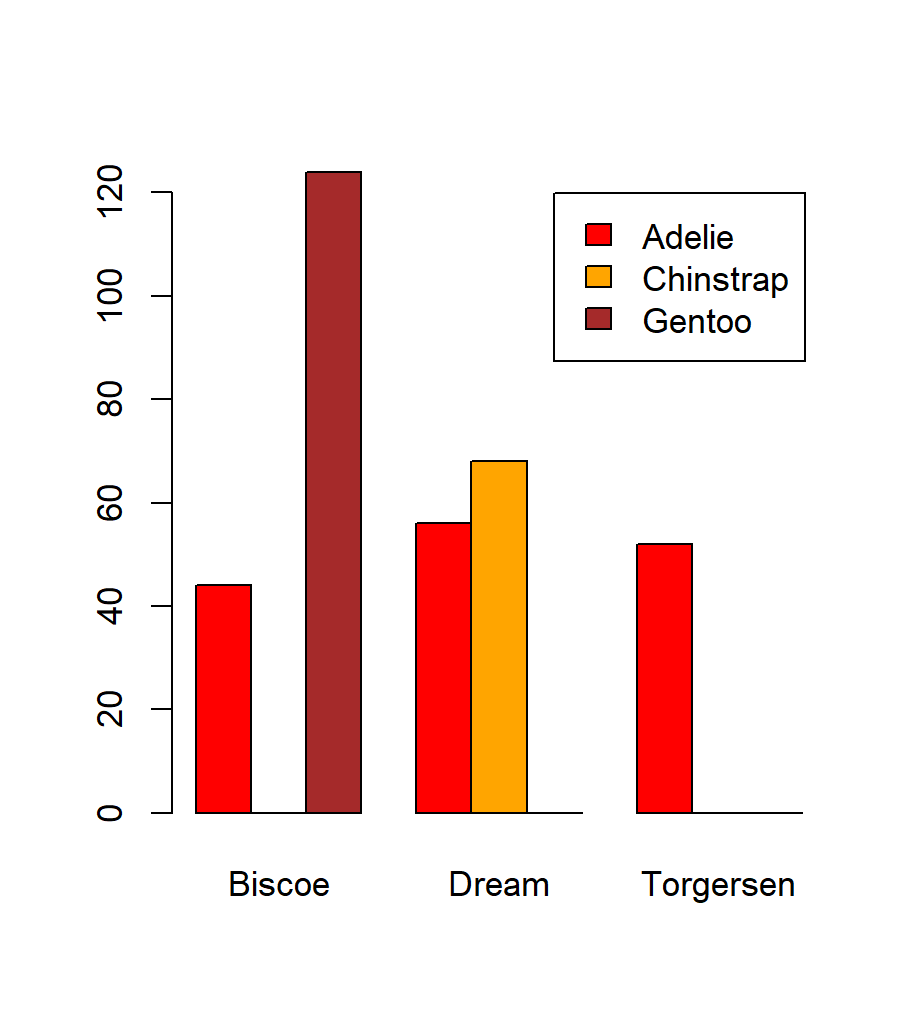
\includegraphics[width=0.5\linewidth]{images/barplot_2_var}
\end{center}



Los gráficos de sectores también pueden ayudar a comparar la composición de una variable cualitativa entre dos grupos, por ejemplo, la distribución del método de estudio en dos cursos.

\bigskip

\begin{lstlisting}[style=rstyle]
# Un gráfico de sectores por cada isla
frecuencias_biscoe    <- tabla[ ,1]
frecuencias_dream     <- tabla[ ,2]
frecuencias_torgersen <- tabla[ ,3]

islands <- colnames(tabla)
colors <- c("red","orange","brown")

par(mfrow = c(1, 3))
pie(frecuencias_biscoe,    main = islands[1], col = colors)
pie(frecuencias_dream,     main = islands[2], col = colors)
pie(frecuencias_torgersen, main = islands[3], col = colors)
par(mfrow = c(1, 1))
\end{lstlisting}

\begin{center}
	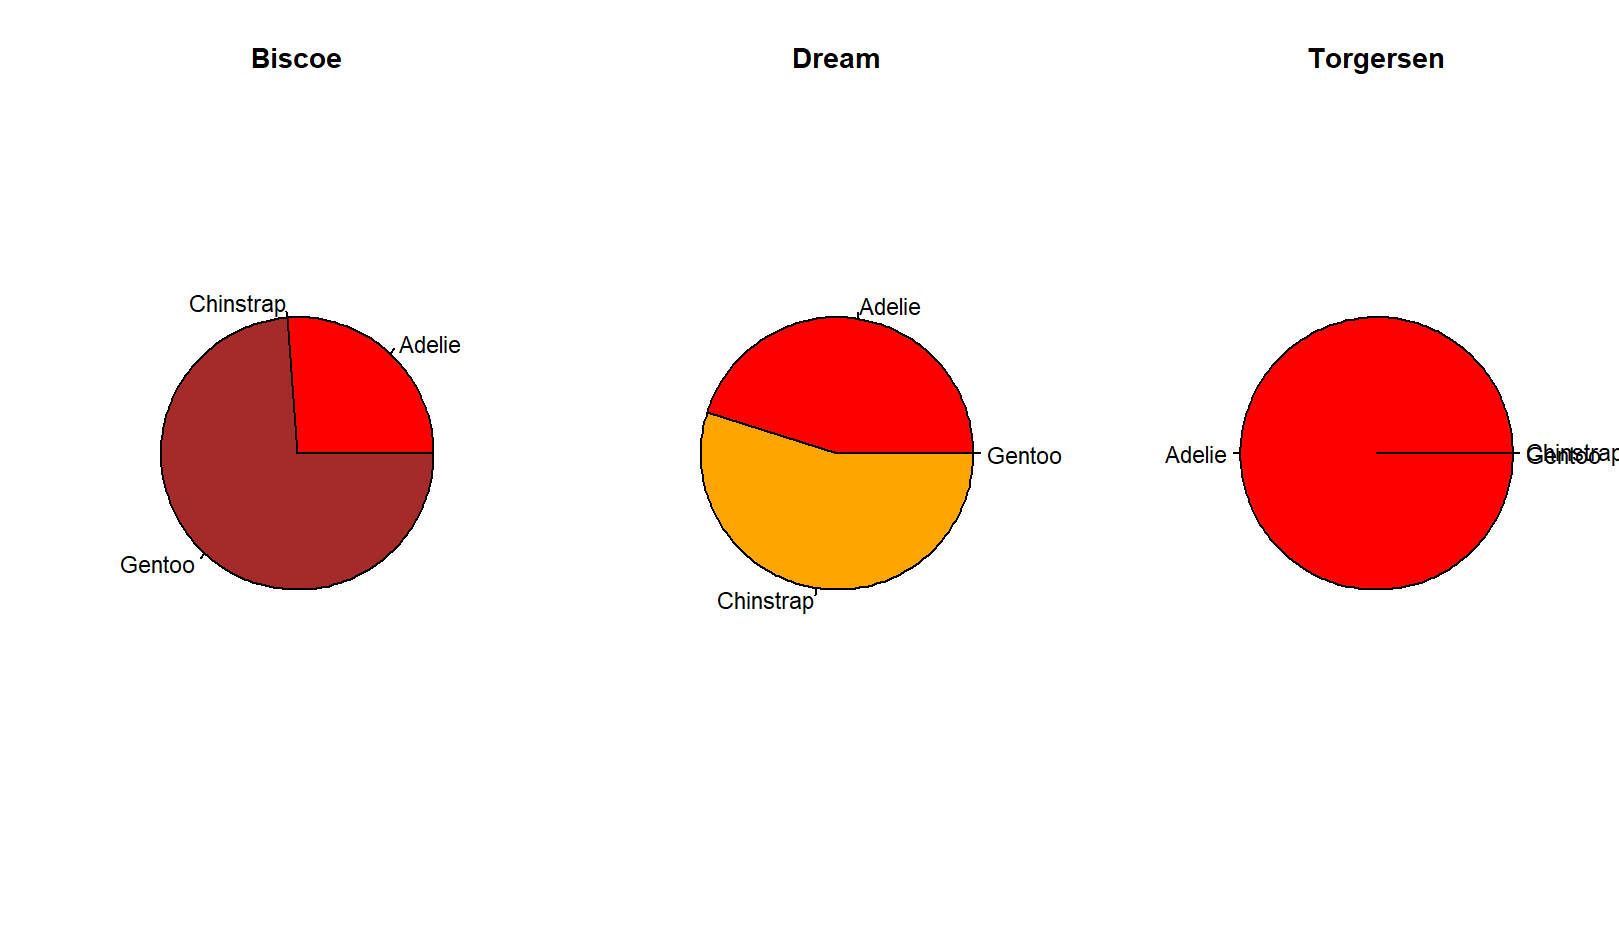
\includegraphics[width=0.95\linewidth]{images/pie_2_var}
\end{center}





\subsection{Una variable cuantitativa y una variable cualitativa nominal}

Se compara la distribución de una variable numérica entre categorías sin orden. Es útil calcular resúmenes (media, mediana y dispersión) por grupo y representarlos con diagramas de caja. Podemos utilizar la función \texttt{aggregate} para ello, especificando en el argumento \texttt{FUN} la función que queremos aplicar.
\begin{lstlisting}[style=rconsole]
> p <- penguins$body_mass
> especie <- penguins$species
> aggregate(p ~ especie, FUN = summary)
\end{lstlisting}

\begin{lstlisting}[style=routput]
    especie   p.Min  p.1st Qu.  p.Median  p.Mean p.3rd Qu. peso.Max
1    Adelie  2850.0     3350.0    3700.0  3700.7    4000.0   4775.0
2 Chinstrap  2700.0     3487.5    3700.0  3733.1    3950.0   4800.0
3    Gentoo  3950.0     4700.0    5000.0  5076.0    5500.0   6300.0
\end{lstlisting}

\noindent Podemos usar gráficos de cajas para realizar una comparación entre los distintos grupos.

\begin{lstlisting}[style=rstyle]
boxplot(penguins$body_mass ~ penguins$species, 
        col = c("red","orange","brown"),
        xlab = "Categoría", 
        ylab = "Variable cuantitativa")
\end{lstlisting}

\begin{center}
	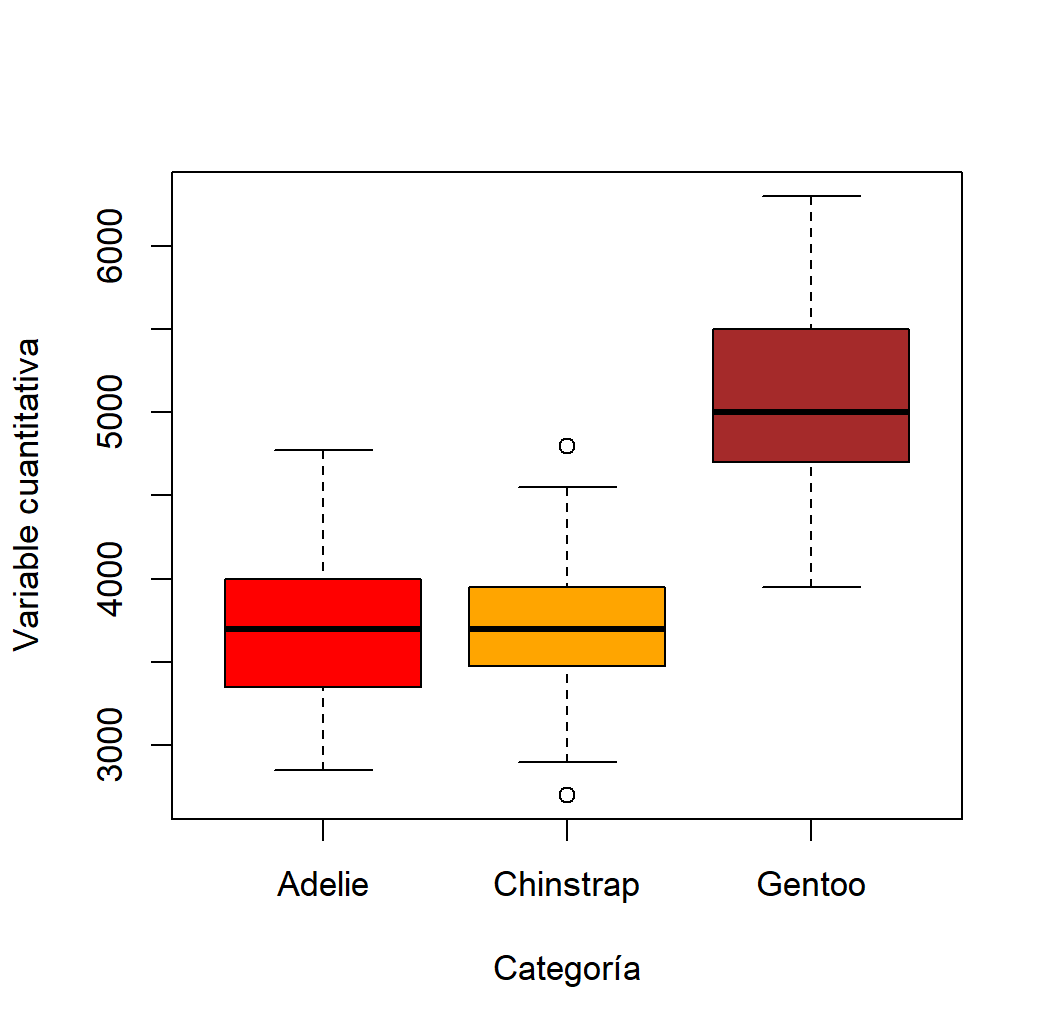
\includegraphics[width=0.5\linewidth]{images/boxplot_2_var}
\end{center}





\subsection{Dos variables cuantitativas: regresión lineal}

Para estudiar la relación entre dos variables cuantitativas se comienza con un diagrama de dispersión. La regresión lineal ajusta una recta que resume una posible tendencia lineal, pero no demuestra causalidad. La pendiente indica el cambio medio estimado en la respuesta por cada unidad adicional de la variable explicativa. 

\medskip

La función \texttt{lm()} (\textit{linear model}) ajusta modelos lineales en \R. En una regresión lineal simple, la fórmula \verb|y ~ x| indica que \texttt{y} es la variable respuesta y \texttt{x} la variable explicativa. El modelo estima una recta de la forma \(\hat{y} = b_0 + b_1 x\), donde \(b_0\) es el intercepto (valor estimado de \texttt{y} cuando \texttt{x = 0}) y \(b_1\) es la pendiente (cambio estimado en \texttt{y} por cada unidad que aumenta \texttt{x}).

\medskip

\begin{lstlisting}[style=rstyle]
# Ajustar el modelo lineal
modelo <- lm(penguins$flipper_len ~ penguins$body_mass)

# Consultar coeficientes, errores estandar, R-cuadrado y pruebas
summary(modelo)

# Coeficientes, valores ajustados y residuos (observado - estimado)
coef(modelo)
fitted(modelo)
residuals(modelo)

# Representar los datos y la recta ajustada
plot(penguins$body_mass, penguins$flipper_len,
     main = "Comparación de la longitud de las alas y el peso",
     xlab = "Peso (g)",
     ylab = "Longitud de las alas")
abline(modelo, col = "red", lwd = 2)
\end{lstlisting}

\begin{center}
	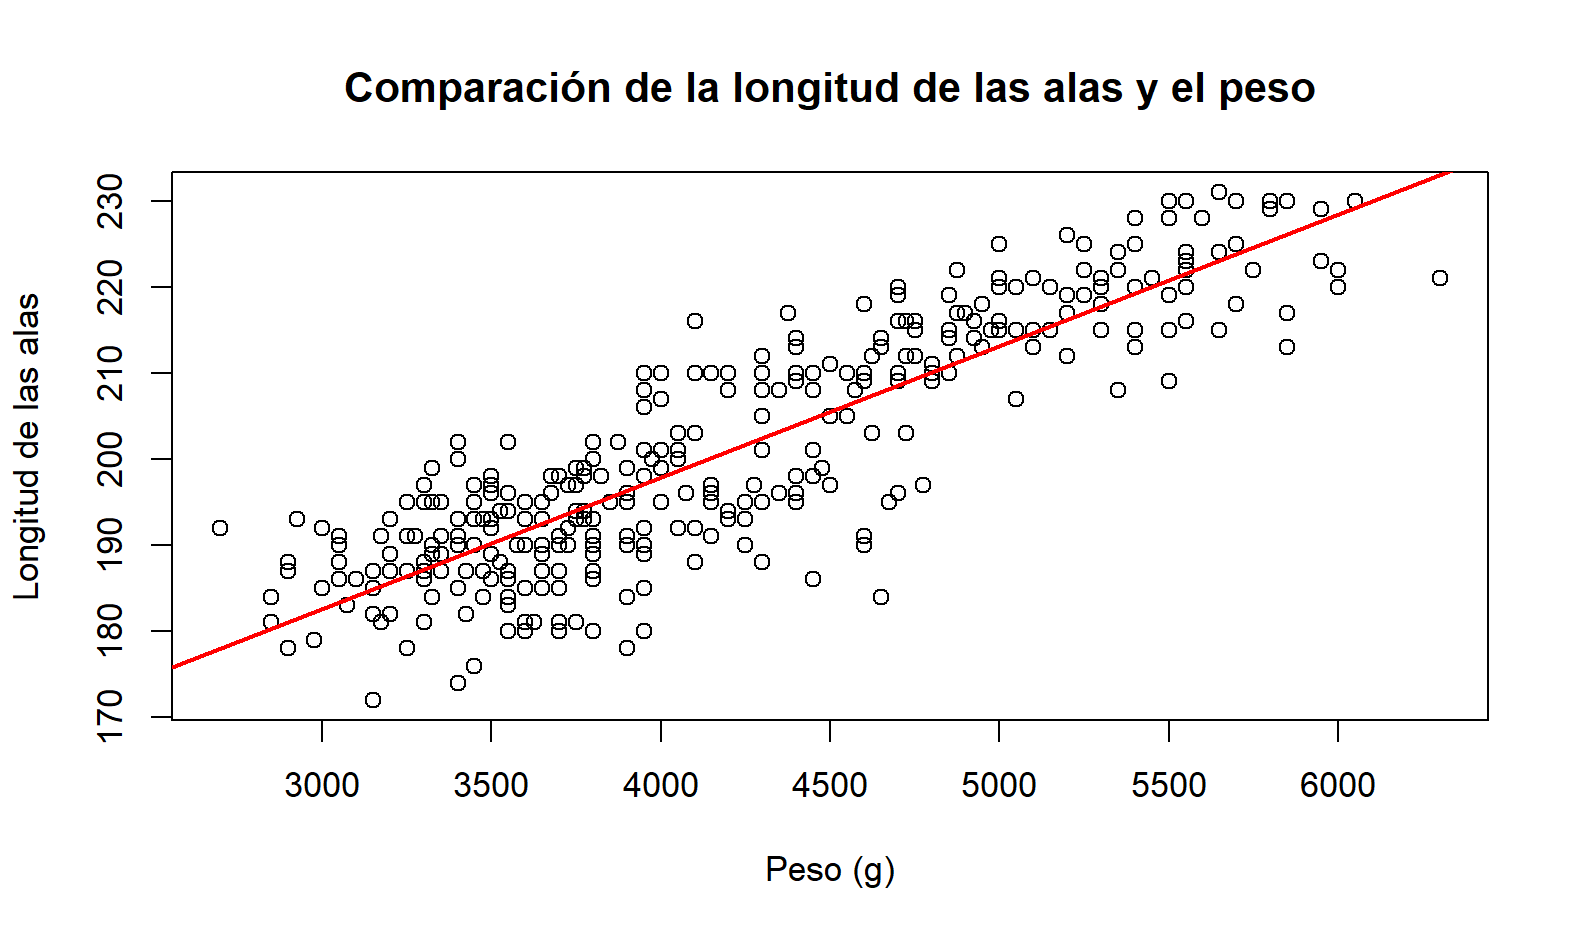
\includegraphics[width=0.75\linewidth]{images/lm}
\end{center}



En \texttt{summary(modelo)}, los coeficientes estimados describen la recta; el valor \(R^2\) indica la proporción de variabilidad de la respuesta explicada por el modelo lineal en la muestra.



\subsection{Gráficos de líneas: evolución temporal}

Los gráficos de líneas son especialmente útiles para representar la evolución de una variable cuantitativa a lo largo del tiempo o de un orden definido. Los puntos se unen para destacar la tendencia; no suelen ser adecuados para categorías nominales sin orden.

\begin{lstlisting}[style=rstyle]
temperaturas <- c(12, 14, 15, 18, 21, 23, 25, 24, 20, 17, 14, 12)
meses <- c("Ene", "Feb", "Mar", "Abr", "May", "Jun",
           "Jul", "Ago", "Sep", "Oct", "Nov", "Dic")
plot(temperaturas,
     type = "b",
     col = "red",
     xlab = "Mes",
     ylab = "Temperatura (grados)",
     main = "Temperatura a lo largo del año")
axis(1, at = seq_along(meses), labels = seq_along(meses))
\end{lstlisting}

\begin{center}
	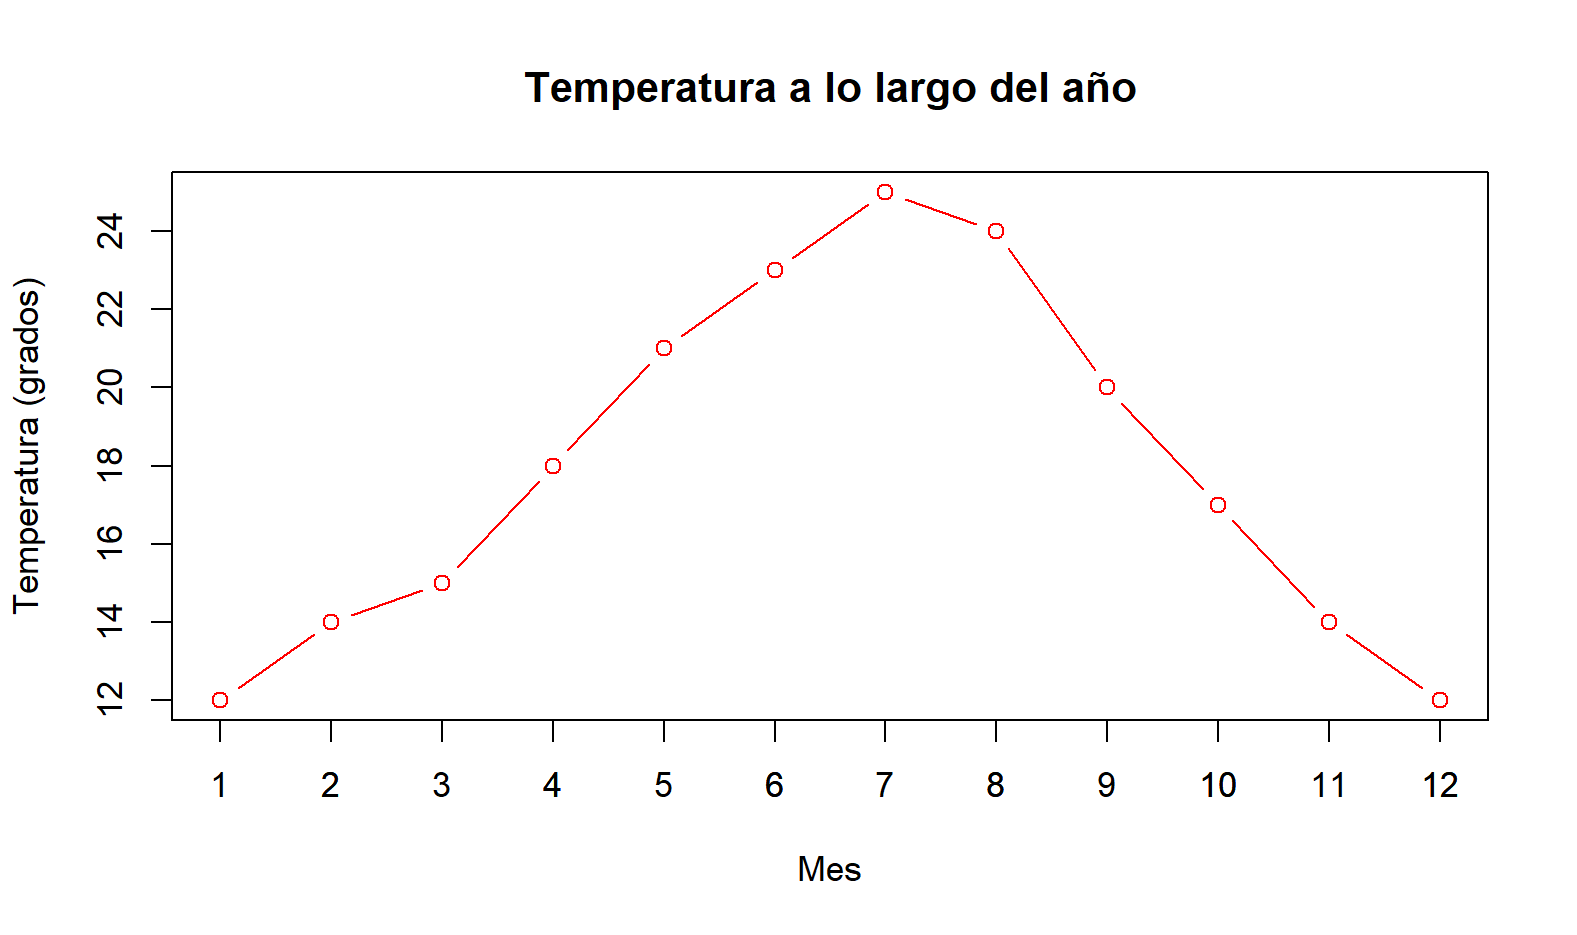
\includegraphics[width=0.75\linewidth]{images/lines}
\end{center}





\section{Ejercicios}

En los ejercicios se pide interpretar los resultados, no solo ejecutar instrucciones. Adapta los nombres de las columnas al conjunto utilizado. Para los análisis de frecuencias, utiliza \texttt{table()} y \texttt{prop.table()}; para los resúmenes cuantitativos, utiliza las funciones descritas en los apartados anteriores. Si una variable contiene valores ausentes, indícalo y utiliza \texttt{na.rm = TRUE} cuando proceda. Los gráficos deben incluir un título y etiquetas comprensibles en los ejes.


\begin{exercise} El fichero \texttt{Datos\_estudiantes.csv}, que puedes encontrar en Blackboard, contiene un conjunto de datos sintéticos acerca del rendimiento de algunos estudiantes de distintos cursos de secundaria. Realiza un análisis estadístico de estos datos. Sigue los pasos siguientes:
\begin{enumerate}
	\item Carga el archivo CSV con \texttt{read.csv(file.choose(), fileEncoding = "UTF-8-BOM")} y guarda el resultado en un objeto llamado \texttt{datos}.

	\item Comprueba que el conjunto de datos se ha cargado bien. Utiliza las funciones \texttt{names()}, \texttt{head()}, \texttt{str()} y \texttt{View()} para comprobar que has cargado bien el conjunto de datos.

	\item Realiza un análisis de frecuencias de las variables cualitativas. Para las variables cuantitativas, calcula una tabla de frecuencias agrupada en intervalos cuando resulte útil. Incluye frecuencias absolutas, relativas y porcentajes.

	\item Obtén las gráficas adecuadas para cada una de las variables cualitativas. 

	\item Realiza un análisis numérico de cada variable cuantitativa: media, mediana, cuartiles, varianza, desviación típica, coeficiente de variación, asimetría y curtosis. Usa \texttt{na.rm = TRUE} cuando corresponda. Comenta los resultados. Comprueba que los datos obtenidos coinciden con aquellos dados por \texttt{summary()} o \texttt{fivenum(x, na.rm = TRUE)}.

	\item Obtén las gráficas adecuadas para cada una de las variables cuantitativas.

	\item Realiza un análisis bivariante de las variables cualitativas \texttt{curso} y \texttt{metodo\_estudio}. Construye una tabla de contingencia y represéntala con un gráfico de barras agrupadas o apiladas.

	\item Realiza un análisis bivariante de la variable cualitativa \texttt{metodo\_estudio} y la variable cuantitativa \texttt{nota\_media}. Compara los resúmenes por grupo y represéntalos mediante diagramas de caja.

	\item Realiza un análisis bivariante de las variables cuantitativas \texttt{horas\_estudio\_semana} y \texttt{nota\_media} mediante regresión lineal. Representa el diagrama de dispersión, ajusta una recta y comenta la pendiente y la fuerza de la relación.
	\end{enumerate}
\end{exercise}






\begin{exercise} El fichero \texttt{Datos\_perros.csv}, que puedes encontrar en Blackboard, contiene un conjunto de datos sintéticos acerca de un estudio sobre perros y el efecto de un nuevo complemento de hierro y vitamina B12 para mejorar los valores de hematocrito. Realiza un análisis estadístico de estos datos. Sigue los pasos siguientes:

\begin{enumerate}
	\item Carga el archivo CSV con \texttt{read.csv(file.choose(), fileEncoding = "UTF-8-BOM")} y guarda el resultado en \texttt{datos}. Comprueba que el archivo contiene las variables \texttt{raza}, \texttt{esteril}, \texttt{leish}, \texttt{hematopre} y \texttt{hematopost}.

	\item Comprueba que el conjunto de datos se ha cargado bien. Utiliza las funciones \texttt{names()}, \texttt{head()}, \texttt{str()} y \texttt{View()} para comprobar que has cargado bien el conjunto de datos.

	\item Realiza un análisis de frecuencias de las variables cualitativas. Para las variables cuantitativas, calcula una tabla de frecuencias agrupada en intervalos cuando resulte útil. Incluye frecuencias absolutas, relativas y porcentajes.

	\item Obtén las gráficas adecuadas para cada una de las variables cualitativas. 

	\item Realiza un análisis numérico de cada variable cuantitativa: media, mediana, cuartiles, varianza, desviación típica, coeficiente de variación, asimetría y curtosis. Usa \texttt{na.rm = TRUE} cuando corresponda. Comenta los resultados. Comprueba que los datos obtenidos coinciden con aquellos dados por \texttt{summary()} o \texttt{fivenum(x, na.rm = TRUE)}.

	\item Obtén las gráficas adecuadas para cada una de las variables cuantitativas.
	
	\item Realiza un análisis bivariante de las variables cualitativas \texttt{raza} y \texttt{leish}. Construye una tabla de contingencia y represéntala con un gráfico de barras agrupadas o apiladas.

	\item Realiza un análisis bivariante de la variable cualitativa \texttt{esteril} y la variable cuantitativa \texttt{hematopost}. Compara los resúmenes por grupo y represéntalos mediante diagramas de caja.

	\item Realiza un análisis bivariante de las variables cuantitativas \texttt{hematopre} y \texttt{hematopost} mediante regresión lineal. Representa el diagrama de dispersión, ajusta una recta y comenta la pendiente y la fuerza de la relación.
	\end{enumerate}
\end{exercise}







\begin{exercise} En este ejercicio haremos un análisis estadístico descriptivo del conjunto de datos \texttt{iris}, que se encuentra en la librería \texttt{datasets} y contiene información acerca de flores de iris. Puedes encontrar información acerca de estos datos en:

\begin{center}
	\url{https://stat.ethz.ch/R-manual/R-devel/library/datasets/html/iris.html}.
\end{center}

Sigue los pasos siguientes:

\begin{enumerate}
	\item Carga el conjunto de datos con \texttt{data(iris, package = "datasets")}.

	\item Comprueba que el conjunto de datos se ha cargado bien. Utiliza las funciones \texttt{names()}, \texttt{head()}, \texttt{str()} y \texttt{View()} para comprobar que has cargado bien el conjunto de datos.

	\item Realiza un análisis de frecuencias de las variables cualitativas. Para las variables cuantitativas, calcula una tabla de frecuencias agrupada en intervalos cuando resulte útil. Incluye frecuencias absolutas, relativas y porcentajes.

	\item Obtén las gráficas adecuadas para cada una de las variables cualitativas. 

	\item Realiza un análisis numérico de cada variable cuantitativa: media, mediana, cuartiles, varianza, desviación típica, coeficiente de variación, asimetría y curtosis. Usa \texttt{na.rm = TRUE} cuando corresponda. Comenta los resultados. Comprueba que los datos obtenidos coinciden con aquellos dados por \texttt{summary()} o \texttt{fivenum(x, na.rm = TRUE)}.

	\item Obtén las gráficas adecuadas para cada una de las variables cuantitativas.

	\item Realiza un análisis bivariante de las variables cualitativas \texttt{Species} y una variable categórica creada agrupando \texttt{Sepal.Length} en dos niveles (por debajo/por encima de la mediana). Construye una tabla de contingencia y represéntala con un gráfico de barras agrupadas o apiladas.

	\item Realiza un análisis bivariante de la variable cualitativa \texttt{Species} y la variable cuantitativa \texttt{Petal.Length}. Compara los resúmenes por grupo y represéntalos mediante diagramas de caja.

	\item Realiza un análisis bivariante de las variables cuantitativas \texttt{Petal.Length} y \texttt{Petal.Width} mediante regresión lineal. Representa el diagrama de dispersión, ajusta una recta y comenta la pendiente y la fuerza de la relación.
	\end{enumerate}
\end{exercise}










\begin{exercise} En este ejercicio haremos un análisis estadístico descriptivo del conjunto de datos \texttt{airquality}, que se encuentra en la librería \texttt{datasets} y contiene información acerca de la calidad del aire en la ciudad de Nueva York entre mayo y septiembre de 1973. Puedes encontrar información acerca de estos datos en:

\begin{center}
	\url{https://stat.ethz.ch/R-manual/R-devel/library/datasets/html/airquality.html}.
\end{center}

Sigue los pasos siguientes:

\begin{enumerate}
	\item Carga el conjunto de datos con \texttt{data(airquality, package = "datasets")} y convierte \texttt{Month} en factor. El conjunto contiene valores ausentes, especialmente en \texttt{Ozone}.

	\item Comprueba que el conjunto de datos se ha cargado bien. Utiliza las funciones \texttt{names()}, \texttt{head()}, \texttt{str()} y \texttt{View()} para comprobar que has cargado bien el conjunto de datos.
	
	\item Realiza un análisis de frecuencias de las variables cualitativas. Para las variables cuantitativas, calcula una tabla de frecuencias agrupada en intervalos cuando resulte útil. Incluye frecuencias absolutas, relativas y porcentajes.
	
	\item Obtén las gráficas adecuadas para cada una de las variables cualitativas. 

	\item Realiza un análisis numérico de cada variable cuantitativa: media, mediana, cuartiles, varianza, desviación típica, coeficiente de variación, asimetría y curtosis. Usa \texttt{na.rm = TRUE} cuando corresponda. Comenta los resultados. Comprueba que los datos obtenidos coinciden con aquellos dados por \texttt{summary()} o \texttt{fivenum(x, na.rm = TRUE)}.

	\item Obtén las gráficas adecuadas para cada una de las variables cuantitativas.
	
	\item Realiza un análisis bivariante de las variables cualitativas \texttt{Month} y una variable categórica creada a partir de \texttt{Temp} (por debajo/por encima de la mediana). Construye una tabla de contingencia y represéntala con un gráfico de barras agrupadas o apiladas.

	\item Realiza un análisis bivariante de la variable cualitativa \texttt{Month} y la variable cuantitativa \texttt{Temp}. Compara los resúmenes por grupo y represéntalos mediante diagramas de caja.

	\item Realiza un análisis bivariante de las variables cuantitativas \texttt{Wind} y \texttt{Ozone} mediante regresión lineal. Representa el diagrama de dispersión, ajusta una recta y comenta la pendiente y la fuerza de la relación.
	\end{enumerate}
\end{exercise}










\begin{exercise} En este ejercicio haremos un análisis estadístico descriptivo del conjunto de datos \texttt{Cars93}, que se encuentra en la librería \texttt{MASS} y contiene información sobre los coches en venta en Estados Unidos en 1993. Puedes encontrar información acerca de estos datos en:

\begin{center}
	\url{https://stat.ethz.ch/R-manual/R-devel/library/MASS/html/Cars93.html}
\end{center}	

Sigue los pasos siguientes:

\begin{enumerate}
	\item Carga el conjunto de datos con \texttt{library(MASS)} y \texttt{data(Cars93)}. Si no está instalado, ejecuta antes \texttt{install.packages("MASS")}.

	\item Comprueba que el conjunto de datos se ha cargado bien. Utiliza las funciones \texttt{names()}, \texttt{head()}, \texttt{str()} y \texttt{View()} para comprobar que has cargado bien el conjunto de datos.

	\item Realiza un análisis de frecuencias de las variables cualitativas. Para las variables cuantitativas, calcula una tabla de frecuencias agrupada en intervalos cuando resulte útil. Incluye frecuencias absolutas, relativas y porcentajes.

	\item Obtén las gráficas adecuadas para cada una de las variables cualitativas. 

	\item Realiza un análisis numérico de cada variable cuantitativa: media, mediana, cuartiles, varianza, desviación típica, coeficiente de variación, asimetría y curtosis. Usa \texttt{na.rm = TRUE} cuando corresponda. Comenta los resultados. Comprueba que los datos obtenidos coinciden con aquellos dados por \texttt{summary()} o \texttt{fivenum(x, na.rm = TRUE)}.

	\item Obtén las gráficas adecuadas para cada una de las variables cuantitativas.

	\item Realiza un análisis bivariante de las variables cualitativas \texttt{Type} y \texttt{Origin}. Construye una tabla de contingencia y represéntala con un gráfico de barras agrupadas o apiladas.

	\item Realiza un análisis bivariante de la variable cualitativa \texttt{Type} y la variable cuantitativa \texttt{Price}. Compara los resúmenes por grupo y represéntalos mediante diagramas de caja.

	\item Realiza un análisis bivariante de las variables cuantitativas \texttt{Horsepower} y \texttt{Price} mediante regresión lineal. Representa el diagrama de dispersión, ajusta una recta y comenta la pendiente y la fuerza de la relación.
	\end{enumerate}
\end{exercise}


\section{README}

Crea un fichero \texttt{README.md} que explique brevemente:

\begin{itemize}
\item el objetivo de la práctica;
\item los datos utilizados en el ejercicio final;
\item qué gráficos se han realizado;
\item qué información proporciona cada gráfico;
\item las principales conclusiones obtenidas.
\end{itemize}

Incluye también una breve reflexión sobre qué tipo de gráfico consideras más adecuado para representar diferentes tipos de información y por qué.

\section*{Entrega}

La práctica deberá entregarse en la fecha acordada con el profesor. Se deberá entregar:
\begin{itemize}
\item el fichero \texttt{.R} con el código de la práctica;
\item el fichero \texttt{README.md};
\item los datos utilizados, si se han obtenido de un fichero externo;
\item cualquier otro fichero necesario para reproducir los resultados.
\end{itemize}
El código deberá ejecutarse correctamente desde el principio hasta el final.



\end{document}



